\documentclass[11pt,a4paper]{article}

% --- Encoding & language ---
\usepackage[utf8]{inputenc}
\usepackage[T1]{fontenc}
\usepackage[english]{babel}

% --- Page layout ---
\usepackage[a4paper,margin=2.5cm]{geometry}
\usepackage{setspace}
\usepackage{parskip}

% --- Math ---
\usepackage{amsmath, amssymb, amsthm}

% --- Figures & tables ---
\usepackage{graphicx}
\usepackage{float}
\usepackage{caption}
\usepackage{subcaption}
\usepackage{booktabs}
\usepackage{array}
\usepackage{multirow}
\usepackage{longtable}

% --- Code listings ---
\usepackage{listings}
\usepackage{xcolor}

% --- References & links ---
\usepackage[numbers]{natbib}
\usepackage{hyperref}
\hypersetup{colorlinks=true, linkcolor=blue, citecolor=blue, urlcolor=blue}
\usepackage{verbatim}
% --- Title ---
\title{Classical Machine Learning Assignment Report}
\author{Diego García Tripiana}
\date{\today}

\begin{document}
\maketitle

\section{Introduction}

In this report we apply classical machine learning techniques to a subset of the
diabetic patient records studied by Strack \emph{et al.}~\cite{strack2014}.

The concrete task addressed in this report is a binary classification problem:
given the information collected during a hospital encounter for a diabetic patient,
predict the value of the \texttt{readmitted} label (\textsc{yes} / \textsc{no}). The
data provided contains 5000 patients described by 37 candidate features that mix
demographics (race, gender, age range), encounter information (admission and
discharge codes, length of stay, number of procedures and medications), diagnosis
codes (ICD-9), and indicators of diabetes-specific medications.

\section{Dataset Description}

Exploring the dataset revealed that it contains 5000 rows and 38 columns.
The target variable is \texttt{readmitted}, which indicates whether the
patient was readmitted to the hospital in the future.
The dataset rows and columns are described in Table \ref{tab:columns}.

\begin{table}[htbp]
\centering
\caption{Variables in the raw dataset (5000 patients $\times$ 38 columns). The 15
medication columns share the same type and meaning, so they are grouped into a single row.}
\label{tab:columns}
\scriptsize
\setlength{\tabcolsep}{6pt}
\renewcommand{\arraystretch}{1.05}
\begin{tabular}{@{}lll@{}}
\toprule
\textbf{Column(s)} & \textbf{Type} & \textbf{Description} \\
\midrule
\texttt{Unnamed: 0}, \texttt{patient\_nbr}           & int   & Row index and patient identifier \\
\texttt{race}, \texttt{gender}                       & cat.  & Demographics \\
\texttt{age}                                         & cat.  & Age range, ordinal (\texttt{[0-10)} \ldots\ \texttt{[90-100)}) \\
\texttt{admission\_type\_id}                          & int   & Coded type of admission \\
\texttt{discharge\_disposition\_id}                   & int   & Coded discharge disposition \\
\texttt{admission\_source\_id}                        & int   & Coded source of admission \\
\texttt{time\_in\_hospital}                           & int   & Length of stay (days) \\
\texttt{num\_lab\_procedures}                         & int   & Number of lab procedures \\
\texttt{num\_procedures}                              & int   & Number of non-lab procedures \\
\texttt{num\_medications}                             & int   & Number of distinct medications \\
\texttt{number\_outpatient}                           & int   & Outpatient visits in the previous year \\
\texttt{number\_emergency}                            & int   & Emergency visits in the previous year \\
\texttt{number\_inpatient}                            & int   & Inpatient visits in the previous year \\
\texttt{number\_diagnoses}                            & int   & Number of diagnoses entered \\
\texttt{diag\_1}, \texttt{diag\_2}, \texttt{diag\_3}  & float & Primary and secondary diagnoses (ICD-9 codes) \\
\texttt{diag\_4}                                      & float & Extra column, not in the original dataset \\
15 medication columns                                 & cat.  & Drug status: \texttt{No}/\texttt{Down}/\texttt{Steady}/\texttt{Up} \\
\texttt{change}                                       & cat.  & Whether the medication was changed \\
\texttt{diabetesMed}                                  & cat.  & Whether any diabetes medication was prescribed \\
\texttt{readmitted}                                   & cat.  & \textbf{Target}: \textsc{yes} / \textsc{no} \\
\bottomrule
\end{tabular}
\end{table}

As we have said, the column to predict is \texttt{readmitted}. We check how balanced the two classes are (YES/NO), because
a strong imbalance would change which metrics and techniques are appropriate. We find 2718 NO (54$\%$) and 2282 YES (46$\%$), which is balanced.
So we can proceed with standard classification techniques without needing special handling for class imbalance.

\section{Data Exploration and Pre-processing}

This dataset uses the string '?' as a
placeholder so  we inspect every categorical column to find these placeholders.
Doing this analysis we find that the columns \texttt{race} and \texttt{tolbutamide} contains this placeholder.
In the case of \texttt{race} we have 112 entries with '?', which is 2.24$\%$ of the data. Since this column already has
an 'Other' category, we merge the unknown patients into it, preserving all 5000 rows.
In the case of \texttt{tolbutamide} we have 3993 entries with '?', which is 79.86$\%$ of the data. As this column only contains
'?' and 'No', replacing the placeholder would yield a near-constant column,
so we just drop the column as it does not provide any information.

Next step is to check for other constant or almost constant columns.
Here we find that the columns
\texttt{acetohexamide}, \texttt{troglitazone}, \texttt{examide} and \texttt{metformin-rosiglitazone} are constant,
so we can drop them. Also the columns \texttt{chlorpropamide}, \texttt{tolazamide} and \texttt{glipizide-metformin} are almost
constant, so we can drop them as well. We can also drop \texttt{Unnamed: 0} and \texttt{patient\_nbr} as they are just identifiers and
do not provide any useful information for the prediction.

There is a suspicious column called \texttt{diag\_4} that was not in the original dataset description.
Comparing for example with the \texttt{diag\_3} column, the diagnosis codes are typically integers, while for \texttt{diag\_4} we have floats.
As we can see in Table~\ref{tab:diag4-corr}, \texttt{diag\_4} is essentially a noisy duplicate of \texttt{diag\_2} (correlation $\approx 0.895$) and is uncorrelated with the target.
Since it is not in the original dataset and is highly redundant with \texttt{diag\_2}, we drop it.

\begin{table}[htbp]
\centering
\caption{Pearson correlation of \texttt{diag\_4} with the other diagnosis columns and with the target.}
\label{tab:diag4-corr}
\begin{tabular}{@{}lc@{}}
\toprule
\textbf{Pair} & \textbf{Correlation} \\
\midrule
\texttt{diag\_4} -- \texttt{diag\_1}     & 0.009 \\
\texttt{diag\_4} -- \texttt{diag\_2}     & \textbf{0.895} \\
\texttt{diag\_4} -- \texttt{diag\_3}     & 0.084 \\
\texttt{diag\_4} -- \texttt{readmitted}  & 0.014 \\
\bottomrule
\end{tabular}
\end{table}


For these diagnostic columns we have a lot of different values, so we use the standard ICD-9 chapter ranges\footnote{ICD-9 chapter ranges: \url{https://en.wikipedia.org/wiki/List_of_ICD-9_codes}.} to map each code to a broad medical category,
producing 16-category columns that we name as \texttt{diag\_x\_cat}.

After this pre-processing step we are left with 26 feature columns, and we are ready to encode
the feature ($x$) variables. We distinguish three types of features:

\begin{itemize}
    \item Numeric features(8): standardised with \texttt{StandardScaler}.
    \item Ordinal feature (1): the \texttt{age} range, encoded with \texttt{OrdinalEncoder} following the natural order of the age intervals.
    \item Nominal features (17): one-hot encoded with \texttt{OneHotEncoder}.
\end{itemize}

 The target variable ($y$) is
binary, so we encode it as 0 for \textsc{no} and 1 for \textsc{yes}.


\begin{comment}
\medskip
Beyond this structural cleaning, we also explored the data visually to anticipate which
features might be predictive. Comparing the distribution of each numeric feature for
readmitted and non-readmitted patients, most features look very similar for the two
classes, but \texttt{number\_inpatient}, \texttt{number\_emergency} and
\texttt{number\_diagnoses} are shifted towards higher values for readmitted patients,
which suggests they carry predictive signal.

Figure~\ref{fig:readmit-rate} shows the readmission rate within each category of several
categorical features. The rate increases steadily with \texttt{age} and is higher for
patients who are on diabetes medication or whose medication was changed, whereas
\texttt{gender} and \texttt{race} show almost flat rates and therefore little signal.

\begin{figure}[htbp]
\centering
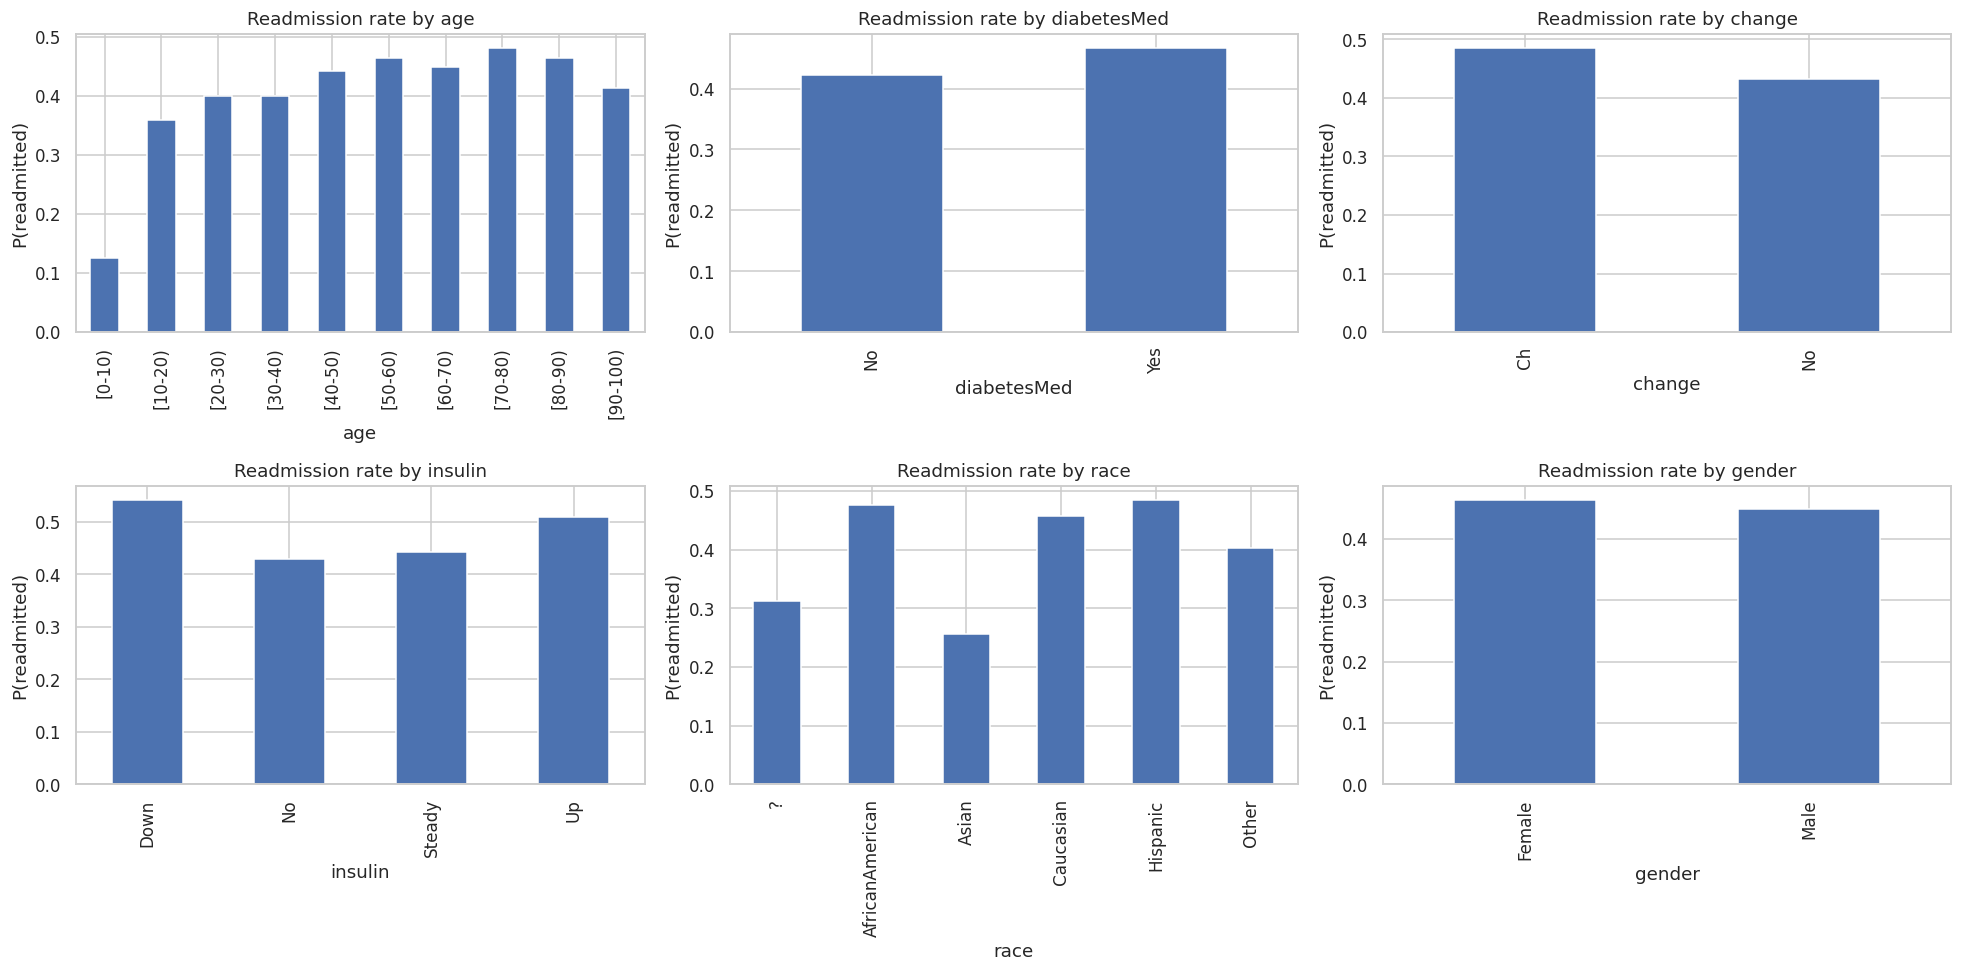
\includegraphics[width=0.82\linewidth]{figures/readmission_rate.png}
\caption{Readmission rate within each category of selected categorical features.}
\label{fig:readmit-rate}
\end{figure}

We also checked the Pearson correlation matrix of the numeric features (not shown): no
pair of features is strongly correlated, so there is no redundancy among them to remove.
\end{comment}

\section{Results}

\subsection{Experimental setup}

Before training any model, we split the data into a training set (80\%, 4000 patients)
and a test set (20\%, 1000 patients). The split is \emph{stratified} on the
target so both sets keep the same class balance, and a fixed random seed
(\texttt{random\_state = 42}) makes the whole experiment reproducible.

We compare a majority-class baseline against seven classical classifiers:

\begin{itemize}
    \item Dummy classifier: always predicts the majority class (\textsc{no}). It only provides a floor that any useful model must beat.
    \item Logistic regression: a linear model that estimates the probability of the positive class.
    \item $k$-nearest neighbours (KNN): classifies each patient by the majority vote of its closest neighbours.
    \item Gaussian naive Bayes: a probabilistic classifier that assumes the features are independent given the class.
    \item Decision tree: a single tree of yes/no rules.
    \item Support vector machine (SVM): finds a maximum margin boundary in a non-linear feature space.
    \item Random forest: an ensemble that averages many decision trees trained on bootstrap samples.
    \item Gradient boosting: an ensemble that builds trees sequentially, each one correcting the errors of the previous ones.
\end{itemize}

Each model is evaluated with 5 fold stratified cross validation on the training
set. We report three metrics: accuracy (fraction of correct predictions,
meaningful here because the classes are balanced), the F1-score of the positive
class (the harmonic mean of precision and recall for the \textsc{yes} class), and
ROC-AUC (the area under the ROC curve, a threshold independent measure of how well
the model ranks patients by risk). ROC-AUC is used as the primary metric for model
selection.

\subsection{Model comparison}

Table~\ref{tab:cv-results} reports the cross-validated results, and
Figure~\ref{fig:roc-all} overlays the ROC curve of every model.

\begin{table}[htbp]
\centering
\caption{5-fold stratified cross-validation results on the training set (mean $\pm$ std), sorted by ROC-AUC.}
\label{tab:cv-results}
\begin{tabular}{@{}lccc@{}}
\toprule
\textbf{Model} & \textbf{Accuracy} & \textbf{F1 (YES)} & \textbf{ROC-AUC} \\
\midrule
SVM (RBF)              & 0.632 $\pm$ 0.009 & 0.484 $\pm$ 0.010 & \textbf{0.677 $\pm$ 0.015} \\
Gradient Boosting      & \textbf{0.633 $\pm$ 0.008} & 0.539 $\pm$ 0.013 & 0.674 $\pm$ 0.010 \\
Logistic Regression    & 0.630 $\pm$ 0.018 & 0.539 $\pm$ 0.021 & 0.672 $\pm$ 0.011 \\
Random Forest          & 0.624 $\pm$ 0.017 & 0.544 $\pm$ 0.016 & 0.665 $\pm$ 0.015 \\
KNN                    & 0.573 $\pm$ 0.012 & 0.481 $\pm$ 0.023 & 0.599 $\pm$ 0.010 \\
Naive Bayes            & 0.493 $\pm$ 0.006 & \textbf{0.636 $\pm$ 0.004} & 0.557 $\pm$ 0.009 \\
Decision Tree          & 0.551 $\pm$ 0.021 & 0.511 $\pm$ 0.019 & 0.548 $\pm$ 0.020 \\
\midrule
Dummy (majority class) & 0.544 $\pm$ 0.000 & 0.000 $\pm$ 0.000 & 0.500 $\pm$ 0.000 \\
\bottomrule
\end{tabular}
\end{table}

\begin{figure}[htbp]
\centering
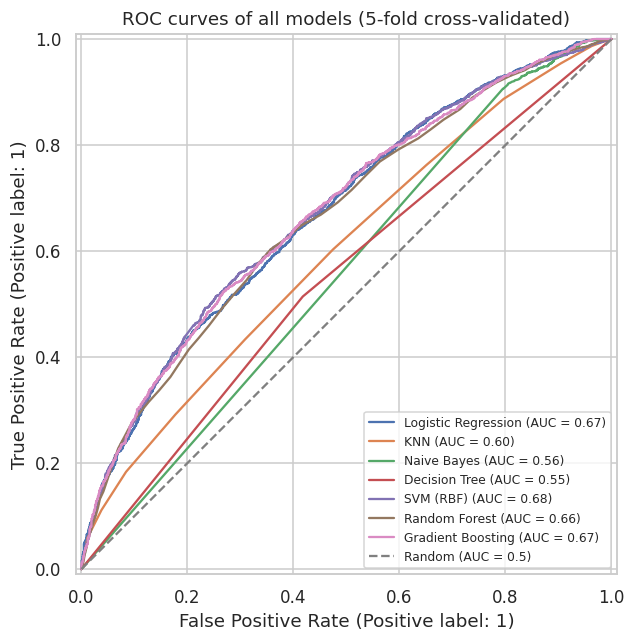
\includegraphics[width=0.52\linewidth]{figures/roc_all_models.png}
\caption{ROC curves of all models, computed from cross-validated predictions on the training set. The dashed diagonal corresponds to a random classifier.}
\label{fig:roc-all}
\end{figure}

Three groups of models can be distinguished. The strongest group (SVM
, gradient boosting and logistic regression) reaches a ROC-AUC of about
0.67-0.68. The random forest, with its default hyper-parameters, performs slightly
below them. Finally, KNN, naive Bayes and the decision tree form a clearly weaker group.
The decision tree overfits the training folds and ends up
close to random (ROC-AUC 0.55). Naive Bayes shows an interesting
pattern: it has the lowest accuracy -(even below the majority class baseline+)
yet the highest F1-score, because it predicts the positive class very often (high
recall, but many false positives). Its feature independence assumption is badly violated
by the one-hot encoded columns. With the exception of the decision tree, every model
clearly beats the baseline ROC-AUC of 0.5, confirming that they extract real signal from
the data.

\subsection{Hyper-parameter tuning}

The two ensemble models (random forest and gradient boosting) were the most promising,
so we tuned them with an exhaustive grid search . The explored grids are listed in
Table~\ref{tab:grids}.

\begin{table}[htbp]
\centering
\caption{Hyper-parameter grids explored with \texttt{GridSearchCV}.}
\label{tab:grids}
\footnotesize
\begin{tabular}{@{}lll@{}}
\toprule
\textbf{Model} & \textbf{Hyper-parameter} & \textbf{Values} \\
\midrule
\multirow{3}{*}{Random Forest}
 & \texttt{n\_estimators}      & 200, 400 \\
 & \texttt{max\_depth}         & None, 10, 20 \\
 & \texttt{min\_samples\_leaf} & 1, 5 \\
\addlinespace
\multirow{3}{*}{Gradient Boosting}
 & \texttt{n\_estimators}  & 200, 400 \\
 & \texttt{learning\_rate} & 0.05, 0.1 \\
 & \texttt{max\_depth}     & 2, 3 \\
\bottomrule
\end{tabular}
\end{table}

The best configurations found were:

\begin{itemize}
    \item Random forest: \texttt{n\_estimators = 400}, \texttt{max\_depth = 10}, \texttt{min\_samples\_leaf = 1}, reaching a cross-validated ROC-AUC of \textbf{0.679}.
    \item Gradient boosting: \texttt{n\_estimators = 200}, \texttt{learning\_rate = 0.05}, \texttt{max\_depth = 2}, reaching a cross-validated ROC-AUC of \textbf{0.676}.
\end{itemize}

Limiting the depth of the random forest (from unbounded to 10) noticeably improves it,
raising its ROC-AUC from 0.665 to 0.679 and making it the best model overall. We
therefore select the tuned random forest as our final model.

\subsection{Final evaluation on the test set}
\label{sec:final-eval}

We now evaluate the tuned random forest onceon the test set, which it
has never seen. The results are summarised in Table \ref{tab:test-results} and
Figure \ref{fig:confusion-roc}.

\begin{table}[htbp]
\centering
\caption{Performance of the tuned random forest on the held-out test set (1000 patients).}
\label{tab:test-results}
\begin{tabular}{@{}lccc@{}}
\toprule
\textbf{Class} & \textbf{Precision} & \textbf{Recall} & \textbf{F1-score} \\
\midrule
\textsc{no} (not readmitted) & 0.63 & 0.80 & 0.71 \\
\textsc{yes} (readmitted)    & 0.65 & 0.45 & 0.53 \\
\midrule
\multicolumn{4}{l}{Accuracy $= 0.64$ \qquad ROC-AUC $= 0.696$} \\
\bottomrule
\end{tabular}
\end{table}

\begin{figure}[htbp]
\centering
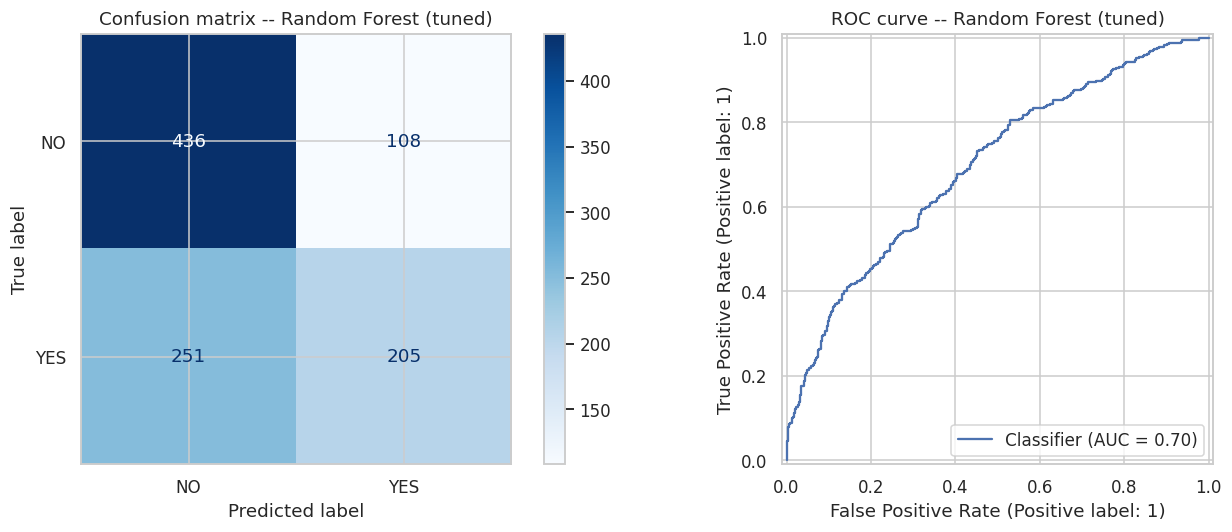
\includegraphics[width=0.9\linewidth]{figures/confusion_roc.png}
\caption{Tuned random forest on the test set: confusion matrix (left) and ROC curve (right).}
\label{fig:confusion-roc}
\end{figure}

On the test set the model reaches an accuracy of 0.64 and a ROC-AUC of 0.696, consistent
with the cross-validation estimate, which means there is no sign of overfitting. The
confusion matrix reveals that the model identifies
non-readmitted patients well ( 0.80 for the \textsc{no} class) but only catches
about 45\% of the patients who are actually readmitted.
When it does predict a readmission, it is right about 65\% of the time. This
behaviour is typical when the available features only partially explain the outcome.

\subsection{Feature importance}

Finally, we inspect which features the tuned random forest relies on most, using the
impurity-based importance scores. Figure~\ref{fig:importance} shows the fifteen most
important features.

\begin{figure}[htbp]
\centering
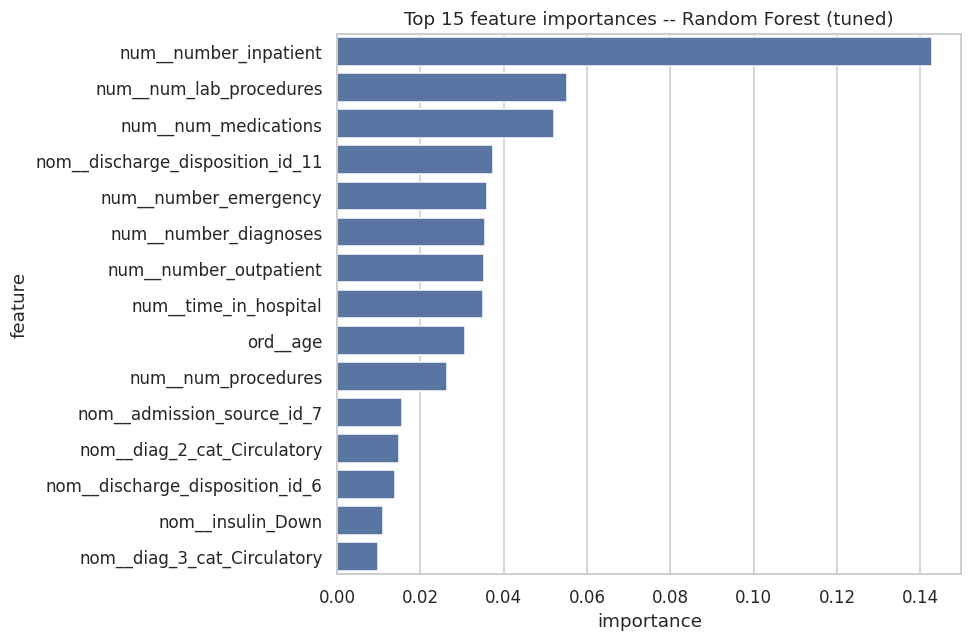
\includegraphics[width=0.66\linewidth]{figures/feature_importance.png}
\caption{Fifteen most important features for the tuned random forest, measured by mean decrease in impurity. The prefixes \texttt{num\_\_}, \texttt{ord\_\_} and \texttt{nom\_\_} indicate the numeric, ordinal and nominal transformer that produced each feature.}
\label{fig:importance}
\end{figure}

The single most important feature, by a large margin, is \texttt{number\_inpatient} ---
the number of inpatient visits in the previous year. It is followed by other measures of
prior hospital utilisation and encounter intensity (\texttt{num\_lab\_procedures},
\texttt{num\_medications}, \texttt{number\_emergency}, \texttt{number\_diagnoses},
\texttt{number\_outpatient}, \texttt{time\_in\_hospital}) together with \texttt{age}.
This is clinically intuitive: patients who have used the hospital intensively in the
recent past, who carry many diagnoses, and who are older are the most likely to be
readmitted. The medication and demographic columns contribute very little.


\begin{thebibliography}{9}
\bibitem{strack2014}
B.~Strack, J.~P. DeShazo, C.~Gennings, J.~L. Olmo, S.~Ventura, K.~J. Cios, and J.~N. Clore,
``Impact of HbA1c Measurement on Hospital Readmission Rates: Analysis of 70,000 Clinical Database Patient Records,''
\emph{BioMed Research International}, vol.~2014, Article ID 781670, 11 pages, 2014.
\end{thebibliography}

\end{document}
